\documentclass[12pt]{article}
\parindent=0.25in

\setlength{\oddsidemargin}{0pt}
\setlength{\textwidth}{440pt}
\setlength{\topmargin}{0in}
\usepackage{amssymb}
\usepackage{amsfonts}
\usepackage{amsmath}
\usepackage{cancel}
\usepackage{latexsym}
\usepackage[center]{subfigure}
\usepackage{epsfig}
\usepackage{3952}
\usepackage{3952-thm}
\usepackage{pstricks,pst-node,pst-tree}
\usepackage{soul, xcolor}
\usepackage{bbold}
\usepackage[backref, colorlinks,citecolor=blue,bookmarks=true]{hyperref}  

\pagestyle{headings}    % Go for customized headings

\newcommand{\handout}[5]{
   \noindent
   \begin{center}
   \framebox{
      \vbox{
    \parbox[t]{4in} {\bf #1 } \vspace{3mm}  {\hfill \bf #2 }
       \vspace{2mm}
       \hbox to 6.00in { {\Large \hfill #5  \hfill} }
       \vspace{1mm}
       \hbox to 6.00in { {\it #3 \hfill #4} }
      }
   }
   \end{center}
   \vspace*{1mm}
}

\hypersetup{linkcolor=magenta}

\begin{document}

\handout{MATH 3952 (Undergraduate Seminar): Quantum Information Theory}{Spring 2024}
{Organizer: Patrick Lei; Presenter: Naomi Jiang}
{Scribe: Mark Chen}{Lecture 5, Talk 1: February 26, 2024}

\thispagestyle{plain}
% \setcounter{section}{-1}
\section*{Chapter 5: Entanglement}
\section{From One Qubit to Two }
\begin{definition}[More Qubits (\textbf{Bipartite}) state]\label{def:2-qubit-state}
The most general form of the two qubits is a normalized linear combination: $$
\Ket{\psi} = c_{00}\Ket{00} + c_{01}\Ket{01} + c_{10}\Ket{10} + c_{11}\Ket{11},
$$ where $c_{00}, c_{01}, c_{10}, c_{11}\in \CC$, so it takes $8$ real parameters to specify. However, we can take out a global factor through normalization, which reduce it to $7$ parameters. Then, since the global phase factor doesn't matter, we now only need $6$ parameters to specify.
\end{definition}

\begin{proposition}
Not all $2$-qubit states can be expressed as $\Ket{a}\Ket{b}$.
\end{proposition}
\begin{proof}
In definition \ref{def:2-qubit-state}, we have already established that it takes $6$ parameters to describe $\Ket{\psi}$. Using the same logic, we would only need to $4$ real parameters to specify the state of $\Ket{a}\Ket{b}$ (two for $\Ket{a}$ and two for $\Ket{b}$), which is strictly less than the $6$ needed for $\Ket{\psi}$.
\end{proof}

\begin{definition}[\textbf{Separable}]
A pair of state vectors where each one pertains to one of the two qubits. For example, $$
\frac{1}{\sqrt{2}} \Ket{00} + \frac{1}{\sqrt{2}}\Ket{01} = \frac{1}{\sqrt{2}} \underset{1\text{st qub.}}{\underbrace{\Ket{0}}} \underset{2\text{nd qub.}}{\underbrace{(\Ket{0} + \Ket{1})}}.
$$
\end{definition}

\begin{definition}[\textbf{Entangled}]
Quantum states that are not \underline{separable} are called \textbf{entangled}. In other words, any bipartite state that cannot be viewed as a pair of two states pertaining to the constituent subsystems is said to be entangled. For example, $$
\frac{1}{\sqrt{2}}\Ket{00} + \frac{1}{\sqrt{2}}\Ket{11}\text{ cannot be written as }\Ket{\psi_1} \Ket{\psi_2}.
$$
\end{definition}

\section{Quantum Theory, Formally (Continued)}
In chapter four, we have discussed formal quantum theoretical primitives like quantum states from Hilbert space, quantum evolutions, quantum circuits, and measurements. Now, we talk about yet another primitive, which is called \textbf{tensor products}, which is the one key part we said we were missing.

\begin{definition}[Tensor Products]
Let $\AAA$ be described by vectors in an $n$-dimensional Hilbert space $\HHH_A$; $\BBB$ an $m$-dimensional $\HHH_B$. Then, the combined system of $\AAA$ and $\BBB$ is then described by vectors in \hl{the $nm$-dimensional tensor product space} $$
\HHH_A \otimes \HHH_B.
$$

\noindent In particular, let $\{\Ket{a_i}\}_{i = 1, \ldots, n}$ be a basis of $\HHH_A$ and $\{\Ket{b_j}\}_{j = 1, \ldots, m}$ be a basis of $\HHH_B$. Then, \hl{the basis of $\HHH_A\otimes \HHH_B$ is} $$
\{\Ket{a_i}\otimes \Ket{b_j}\}_{i\in [n], j\in [m]}.
$$ For brevity, we typically write $$
\Ket{a_i}\otimes \Ket{b_j} = \Ket{a_i}\Ket{b_j} = \Ket{a_ib_j}.
$$

\noindent Also, clearly, the \hl{tensor product space} $$
\HHH_A \otimes \HHH_B = \left\{\underset{i,j}{\sum}c_{ij}\Ket{a_i}\otimes \Ket{b_j}: c_{ij}\in \CC, \Ket{a_i}\in \HHH_A, \Ket{b_j}\in \HHH_B\right\}
$$
\end{definition}

\begin{proposition} Properties of tensor product operation $\otimes$:
\begin{itemize}
    \item (Distributivity) $$
    \begin{aligned}
    \Ket{a}\otimes (\beta_1\Ket{b_1} + \beta_2\Ket{b_2})
        &= \beta_1\Ket{a}\otimes\Ket{b_1} + \beta_2\Ket{a}\otimes \Ket{b_2}\\
    (\alpha_1\Ket{a_1} + \alpha_2\Ket{a_2})\otimes \Ket{b}
        &= \alpha_1\Ket{a_1}\otimes\Ket{b} + \alpha_2\Ket{a_2}\otimes \Ket{b}.
    \end{aligned}
    $$
    \item (Is still a Hilbert space with the same inner product rules) $$
    (\Bra{a'}\otimes \Bra{b'}) (\Ket{a} \otimes \Ket{b}) = \bk{a'}{a}\bk{b'}{b},
    $$ which can be extended by \underline{linearity} to \textbf{sums of tensor products of vectors}, and, by \underline{associativity}, to any number of \textbf{subsystems}.
    \item ($\dag$ operation on it doesn't reverse the order of elements) $$
        (\Ket{a}\otimes \Ket{b})^\dag = \Bra{a} \otimes \Bra{b}.
    $$
\end{itemize}
\end{proposition}

\begin{definition}[\textbf{Separable \& Entangled}] Revisited with definition of tensor product.
\begin{itemize}
    \item (\textbf{Separable}) Sometimes, a joint state $\Ket{\psi}$ can be written as a single tensor product (as compared to multiple), as in $$
    \Ket{\psi} = \Ket{a}\otimes \Ket{b},
    $$ then we are saying that, for $\Ket{\psi}$, its subsystem $\AAA$ is in state $\Ket{a}$ and its subsystem $\BBB$ is in state $\Ket{b}$.

    Because this is the case, we notice that $$
    \begin{aligned}
    \Ket{\psi}
        &= \Ket{a}\otimes \Ket{b}\\
        &= \underset{i,j}{\sum}\alpha_i \Ket{a_i}\otimes \beta_j \Ket{b_j}\\
        &= \underset{i,j}{\sum}(\alpha_i\beta_j) \Ket{a_i}\otimes  \Ket{b_j},
    \end{aligned}
    $$ where $c_{ij} = \alpha_i\beta_j\in \CC$ is a very specific form. This kind of $\Ket{\psi}$ is called separable.
    \item (\textbf{Entangled}) If not separable.
\end{itemize}
\end{definition}

\begin{definition}[Tensor Product of Two Operators]
Let $A$ be an operator on $\HHH_A$, and $B$ an operator on $\HHH_B$. Then, we define \hl{$A\otimes B$ as an operator on $\HHH_A\otimes \HHH_B$} such that $$
(A\otimes B)(\Ket{a}\otimes \Ket{b}) = (A\Ket{a})\otimes (B\Ket{b}),
$$ which can be generalized to all other vectors by linearity: $$
A\otimes B\prt{\underset{i,j}{\sum}c_{ij}\Ket{a_i}\otimes \Ket{b_j}} = \underset{i,j}{\sum}c_{ij}A\Ket{a_i}\otimes B\Ket{b_j}
$$
\end{definition}

\section{More Qubits, and Binary Representations}
A \textbf{classical} register composed of three bits can store only one of the $8$ possible $3$-bit strings. However, a \textbf{quantum register} composed of three qubits can store \textit{any subset of the $8$ $3$-qubit states via superposition}.

\begin{example}
Say, we start with $\Ket{011}$ and apply Hadamard gate to the first qubit: $$
\Ket{011}\overset{H\otimes 1\otimes 1}{\mapsto}\frac{1}{\sqrt{2}}(\Ket{0}+\Ket{1}) \otimes \Ket{1} \otimes \Ket{1} = \frac{1}{\sqrt{2}}(\Ket{011} + \Ket{111})
$$
\end{example}

\begin{example}\label{eg:hadamard-trans}
Note how we can easily get a superposition of all $8$ possible $3$-qubit states:
\begin{center}
    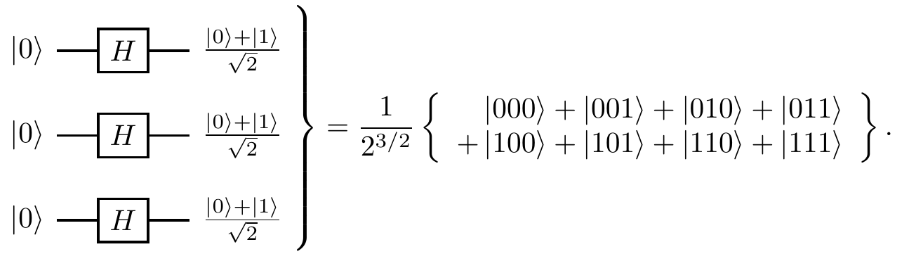
\includegraphics[width = 25em]{images/1.jpg}
\end{center}
\end{example}

\begin{definition}[Hadamard Transform, $H^{\otimes n}$]\label{def:hadamard-trans}
It turns out the operation described in example \ref{eg:hadamard-trans} is very useful: this kind of operations of ``applying the hardamard gate to each of the $n$ qubits" is known as \hl{Hadamard transform}.\\

\noindent Like the Hadamard gate in the typical quantum interference circuit, the Hadamard transform opens (and closes) multi-qubit interference.
\end{definition}

\begin{notation}
As a result of the operation defined in definition \ref{def:hadamard-trans} and exemplified in \ref{eg:hadamard-trans}, we can generally write the outcome of the Hadamard transform on $n$ qubits as: $$
\frac{1}{2^{n/2}}\underset{x\in \{0,1\}^n}{\sum}\Ket{x}.
$$ Furthermore, we can switch to decimal representation of $N = 2^n$: $$
\frac{1}{\sqrt{N}} \Sum{x}{0}{N-1}\Ket{x},
$$ where, obviously, $\Ket{7}$ would represent $\Ket{111}$, and so on.
\end{notation}

\section{Separable / Entangled, Formally}
\begin{proposition}\label{prop:cond-for-separability}
\hl{A joint state $\Ket{\psi}$ in $\HHH_A\otimes \HHH_B$ is separable $\iff$ $\Ket{\phi_i}$ are constant multiples of the same vector (we will define what $\Ket{\phi_i}$ is in expansion (1) in the proof).}
\end{proposition}
\begin{proof}
We can study the restrictions going both ways as follows:
\begin{itemize}
    \item If $\Ket{\psi}$ can be written as $\Ket{\psi} = \Ket{a} \Ket{b}$: First of all, any joint state $\Ket{\psi}$ (i.e. \underline{entangled} or \underline{separable}) can generally be written as
    \begin{equation}
    \Ket{\psi} = \underset{i,j}{\sum}c_{ij}\Ket{a_i}\otimes \Ket{b_j} = \underset{i}{\sum}\Ket{a_i}\otimes \prt{\underset{j}{\sum}c_{ij}\Ket{b_j}} = \underset{i}{\sum}\Ket{a_i}\otimes \Ket{\phi_i},
    \end{equation} where $\Ket{\phi_i} = \prt{\underset{j}{\sum}c_{ij}\Ket{b_j}}$.

    Now, use the assumption that $\Ket{\psi}$ is \underline{separable}:
    \begin{equation}
    \Ket{\psi} = \Ket{a}\otimes \Ket{b} = \underset{i}{\sum}\alpha_i \Ket{a_i} \otimes \Ket{b} = \underset{i}{\sum} \Ket{a_i} \otimes \prt{\alpha_i\Ket{b}}
    \end{equation}

    Combining (1) and (2), we get $$
    \underset{j}{\sum}c_{ij}\Ket{b_j} = \Ket{\phi_i} = \alpha_i\Ket{b},
    $$ which means that each $\Ket{\phi_i}$ is a \underline{constant multiple}e of the same vector $\Ket{b}$.
    \item Conversely, if $\Ket{\phi_i} = \alpha_i \Ket{b},\forall i$ in (1), then $\Ket{\psi}$ must be separable.
\end{itemize}

\noindent Therefore, we have established that $$
\Ket{\psi}\text{ is separable }\iff\Ket{\phi_i}\text{ is a constant multiple of $\Ket{b}$}
$$
\end{proof}

\begin{proposition}\label{prop:entangled-states-are-more-common}
\hl{Most of the joint states in $\HHH_A\otimes \HHH_B$ are entangled: i.e. they cannot be written in the form $\Ket{a}\otimes \Ket{b}$ for some $\Ket{a}\in \HHH_A$ and $\Ket{b}\in \HHH_B$. }
\end{proposition}
\begin{proof}
Clearly, if we choose $\Ket{\psi}$ at random, it is very unlikely that the condition ``$\Ket{\phi_i}$ is a constant multiple of $\Ket{b}$" is satisfied as we have shown in proposition \ref{prop:cond-for-separability}. Here is why:
\begin{itemize}
    \item (Total number of possible $\Ket{\psi}$) Recall what we have established here. For a quantum system with $n$ qubits, we can have a superposition of $2^n$ terms. So, \hl{we can specify, in general, a quantum system with $2\cdot 2^n - 2 = \underline{2(2^n - 1)}$ real parameters} ($2$ for each term in the superposition minus $1$ by normalization and minus another $1$ by ignoring the global phase factor resulting from the normalization).
    \item (Total number of $\Ket{\psi}$ that satisfy the condition in proposition \ref{prop:cond-for-separability}) When it's separable, each term must be a multiple of a single $\Ket{b}$. So \hl{it takes only $\underline{2n}$ real parameters to specify separable joint states}.
\end{itemize}

\noindent So, the space of all separable joint states is much smaller than the space of all joint states in $\HHH_A\otimes \HHH_B$. All the rest of the joint states that cannot be specified by the ways to specify separable states, because proposition \ref{prop:cond-for-separability} is an ``$\iff$" statement, are \textbf{entangled} (which is a lot more because the difference is between exponential and linear in terms of $n$)!
\end{proof}

\begin{remark}[Serge Embedding]
We proved proposition \ref{prop:entangled-states-are-more-common} using counting argument. However, to actually show if a state is separable or not is an \textbf{NP-hard problem}!\\

\noindent To understand the separability problem from a different point of view, one way is to use \underline{algebraic geometry}, using the notion of projective space.\\

\noindent For more details: In Joana Cirici et al's 2020 paper, \href{https://arxiv.org/pdf/2008.09583.pdf}{Characterization of quantum entanglement via a hypercube of Segre embeddings}, she used the above idea to rephrase proposition \ref{prop:cond-for-separability} into algebraic geometric terms: ``A state, $\Ket{\psi}$, of two qubits is separable $\iff$ its corresponding points in $\PP^3$ lies in Serge cavity $\Sigma$."
\end{remark}

\section{Controlled-$\NOT$ (C-$\NOT$)}
If joint states are separable, then nothing too interesting happens: they go through their respective unitary operations and still end up separable in the end.

\begin{center}
    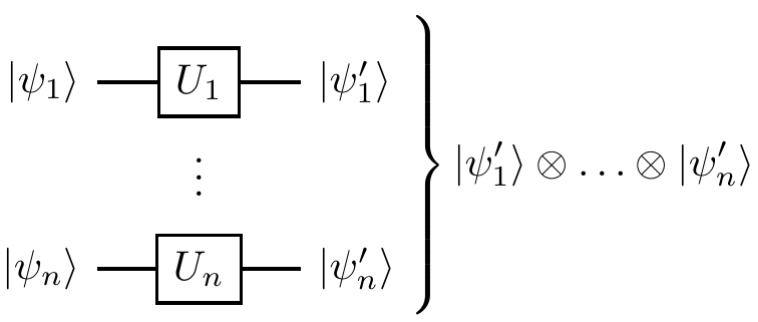
\includegraphics[width = 15em]{images/2.jpg}
\end{center}

\noindent This becomes more interesting when some of the qubits in the initial prepared joint state are entangled! That is, we will have interactions that are no longer just \textit{tensor products of unitary operators on individual qubits}! The most popular such entangling gate is called the Controlled-$\NOT$ gate.

\begin{definition}[Controlled-$\NOT$]\label{def:c-not}
The c-$\NOT$ gate \underline{does nothing if $\Ket{x} = \Ket{0}$} and \underline{flips $\Ket{y}$} \underline{if $\Ket{x} = \Ket{1}$}. As a circuit, it can be visualized as:
\begin{center}
    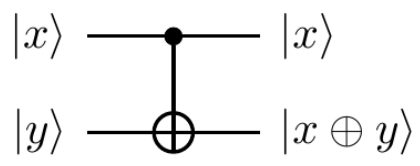
\includegraphics[width = 15em]{images/3.jpg}.
\end{center}
\end{definition}

\begin{notation}
Alternatively, the circuit in definition \ref{def:c-not} can be written as a matrix: $$
\text{c-}\NOT = \begin{bmatrix}
1 & 0 & \vline & 0 & 0 \\
0 & 1 & \vline & 0 & 0 \\
\hline
0 & 0 & \vline & 0 & 1 \\
0 & 0 & \vline & 1 & 0 \\
\end{bmatrix}.
$$

\noindent To use it, we first recall that: $\Ket{00} = \begin{bmatrix}
    1\\
    0\\
    0\\
    0
\end{bmatrix}$, $\Ket{01} = \begin{bmatrix}
    0\\
    1\\
    0\\
    0
\end{bmatrix}$, $\Ket{10} = \begin{bmatrix}
    0\\
    0\\
    1\\
    0
\end{bmatrix}$, and $\Ket{11} = \begin{bmatrix}
    0\\
    0\\
    0\\
    1
\end{bmatrix}$. So, say we operate c-$\NOT$ on $\Ket{10}$ as an input: $$
\text{c-}\NOT \Ket{10} = \begin{bmatrix}
1 & 0 & \vline & 0 & 0 \\
0 & 1 & \vline & 0 & 0 \\
\hline
0 & 0 & \vline & 0 & 1 \\
0 & 0 & \vline & 1 & 0 \\
\end{bmatrix}\begin{bmatrix}
    0\\
    0\\
    1\\
    0
\end{bmatrix} = \begin{bmatrix}
    0\\
    0\\
    0\\
    1
\end{bmatrix} = \Ket{11}.
$$ You can easily verify that the c-$\NOT$ logic works on all of the four possible inputs.
\end{notation}

\begin{notation}
c-$\NOT$ can also be written as a sum of tensor product: $$
\text{c-}\NOT = \kb{0}{0}\otimes \mathbb{1} + \kb{1}{1}\otimes X,
$$ which means that,
\begin{itemize}
    \item (if the first bit is in $\Ket{0}$) then we apply $\mathbb{1}$ to the second bit, which is nothing.
    \item (if the first bit is in $\Ket{1}$) then we apply $X$ (note that it is the Pauli operator $$X = \sigma_X = \begin{bmatrix}
        0 & 1\\
        1 & 0
    \end{bmatrix})$$ to the second bit, which is to swap its state ($\Ket{1}$ to $\Ket{0}$, and $\Ket{0}$ to $\Ket{1}$).
\end{itemize}
\end{notation}

\section{Bell States}
We can generate entangled states quite easily, now that we have \underline{Hadamard gates} and \underline{c-$\NOT$ gates} at our disposal.

\begin{definition}[Generating Entanglements]
The idea is to first apply the Hadamard gate $H$ on the first bit, and then c-$\NOT$ gate on the resulting system. The circuit on an example input, $\Ket{00}$, looks like:
\begin{center}
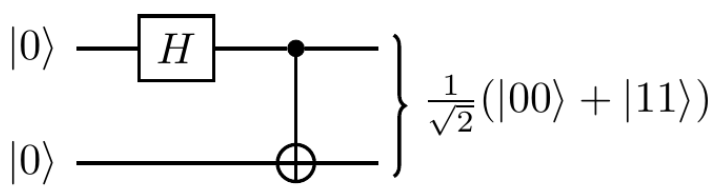
\includegraphics[width = 20em]{images/4.jpg}
\end{center}

\noindent We can write out explicitly for the four possible inputs:$$
\begin{aligned}
\Ket{00} &\overset{H\otimes \mathbb{1}}{\mapsto} \frac{1}{\sqrt{2}}(\Ket{0} + \Ket{1})\Ket{0} = \frac{1}{\sqrt{2}}(\Ket{00} + \Ket{10})\overset{\text{c-}\NOT}{\mapsto}\boxed{\frac{1}{\sqrt{2}}(\Ket{00} + \Ket{11}) =: \Ket{\psi_{00}} = \Phi^+}\\
\Ket{01} &\overset{H\otimes \mathbb{1}}{\mapsto} \frac{1}{\sqrt{2}}(\Ket{0} + \Ket{1})\Ket{1} = \frac{1}{\sqrt{2}}(\Ket{01} + \Ket{11})\overset{\text{c-}\NOT}{\mapsto}\boxed{\frac{1}{\sqrt{2}}(\Ket{01} + \Ket{10}) =: \Ket{\psi_{01}} = \Psi^+}\\
\Ket{10} &\overset{H\otimes \mathbb{1}}{\mapsto} \frac{1}{\sqrt{2}}(\Ket{0} - \Ket{1})\Ket{0} = \frac{1}{\sqrt{2}}(\Ket{00} - \Ket{10})\overset{\text{c-}\NOT}{\mapsto}\boxed{\frac{1}{\sqrt{2}}(\Ket{00} - \Ket{11}) =: \Ket{\psi_{10}} = \Phi^-}\\
\Ket{11} &\overset{H\otimes \mathbb{1}}{\mapsto} \frac{1}{\sqrt{2}}(\Ket{0} - \Ket{1})\Ket{1} = \frac{1}{\sqrt{2}}(\Ket{01} - \Ket{11})\overset{\text{c-}\NOT}{\mapsto}\boxed{\frac{1}{\sqrt{2}}(\Ket{01} - \Ket{10}) =: \Ket{\psi_{11}} = \Psi^-}
\end{aligned}
$$
\end{definition}

\begin{definition}[\textbf{Bell States}]
\hl{$\Phi^+ = \Ket{\psi_{00}}, \Psi^+ = \Ket{\psi_{01}}, \Phi^- = \Ket{\psi_{10}}, \Psi^- = \Ket{\psi_{11}}$ will be the notations we use to denote these very specific circuits from now on!} And, these are the four \textbf{Bell states}.
\end{definition}

\begin{proposition}
\textbf{Bell states} form an \underline{orthonormal basis} in $\HHH_1\otimes \HHH_2$ of two qubits.
\end{proposition}

\begin{remark}
The easiest way to perform measurements in the Bell states is to rotate it to the standard basis and perform measurements there. That is because the entanglement generating operations are unitary operators (which means their \underline{adjoins} are their \underline{inverses}.)\\

\noindent Formally, denote the entanglement generating unitary operator that maps from $\Ket{ij}$ to $\Ket{\psi_{ij}}$ as $U$, i.e. $U\Ket{ij} = \Ket{\psi_{ij}}$. Then, $$
\Bra{\psi_{ij}} = \Ket{\psi_{ij}}^\dag = \Bra{ij}U^\dag.
$$ So, the probability amplitude of starting at $\Ket{ij}$ and end up in $\Ket{\psi_{ij}}$ through the operations is $$
\bk{\psi_{ij}}{ij} = \Bra{ij}U^\dag\Ket{\psi_{ij}}
$$
\end{remark}

\begin{definition}[Maximally Entangled]
The \underline{Bell states} are said to be \textbf{maximally entangled}, which means that their \textbf{reduced density operators} are \underline{maximally mixed} (terms that we will explain in chapter 8).\\

\noindent In terms that we could understand right now, the outcomes of any measurements performing on Bell states are completely random.
\end{definition}


\end{document}